\chapter{Gradients and Their Applications}

\section{Gradient Vectors}
\index{directional derivative}
You are halfway up a mountain in thick fog and want to reach the top as fast
as possible. Which way should you walk? The \newterm{gradient} answers
exactly that question: it is a vector that points in the direction of
steepest ascent. In order to 
understand the gradient, we must first discuss directional derivatives. Recall 
that the partial derivatives, $f_x$ and $f_y$, can be used to define a plane 
tangent to the surface $z = f(x,y)$ (see figure \ref{fig:plane}). Directional 
derivatives allow us to find the slope of the tangent plane in directions 
other than the $x$- and $y$-directions. 

\begin{figure}[H]
    \centering
    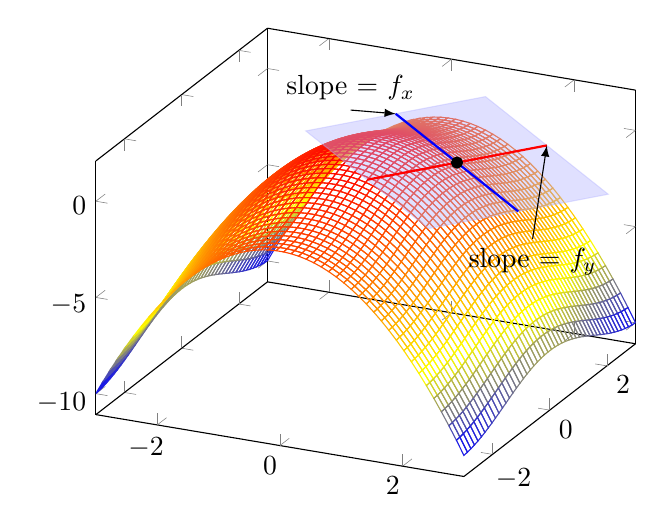
\begin{tikzpicture}
    \begin{axis}[]
        \addplot3[mesh, samples = 50, domain = -3:3]{cos(deg(y)) - x^2};
        \addplot3[black, mark=*] coordinates {(1, 1.047, -0.5)};
        \filldraw[blue!30, opacity = 0.4] (0, -2.094, 4.220) -- 
        (0, 4.189, -1.221) -- (2, 4.189, -5.221) -- (2, -2.094, 0.220) -- cycle;
        \draw[red, thick](1, -2.094, 2.220) -- (1, 4.189, -3.221);
        \draw[latex-] (0, 1.047, 1.5) -- (-0.5, 0.547, 2) node[above] {
        slope = $f_x$};
        \draw[blue, thick](0, 1.047, 1.5) -- (2, 1.047, -2.5);
        \draw[latex-](1, 4.189, -3.221) -- (2, 1.547, -4.5) node[below] {
        slope = $f_y$};
    \end{axis}
    \end{tikzpicture}
    \caption{The partial derivatives $f_x$ and $f_y$ define a tangent 
    plane}
    \label{fig:plane}
\end{figure}

\subsection{Directional Derivatives}
The contour map in figure \ref{fig:mountain} shows the elevation, $f(x, y)$ 
for a mountain. You already know that you can use the partial derivatives, 
$f_x$ and $f_y$ to find the rate of change in elevation going east-west or 
north-south. But what about other directions? Suppose the hiking path you are 
on goes north-east. How can you predict the steepness (i.e. the rate of 
elevation change) along this path? The directional derivative allows us to 
find the rate of change in any direction. 

\begin{figure}[H]
    \centering
    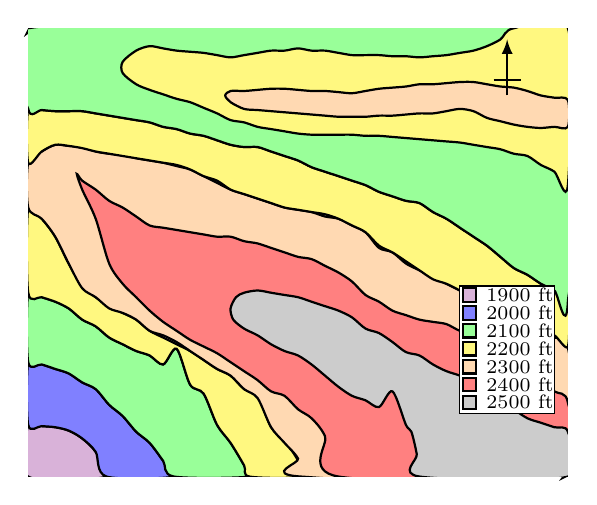
\begin{tikzpicture}
        \begin{axis}[xmin = 0, xmax = 20, ymin = 0, ymax = 20, ticks = none, 
        axis lines = center]
        \draw[fill = violet!30, draw = black, thick] plot[smooth cycle] 
        coordinates {(0, 2.3) (0.5, 2.25) (1, 2.2) (1.5, 2.05) (2, 1.7) 
        (2.5, 1.1) (2.9, 0) (0,0)};
        \draw[fill = blue!50, draw = black, thick] plot[smooth cycle] 
        coordinates {(0, 2.3) (0.5, 2.25) (1, 2.2) (1.5, 2.05) (2, 1.7) 
        (2.5, 1.1) (2.9, 0) (5.4, 0) (5, 0.7) (4.5, 1.5) (4, 2) (3.5, 2.7) 
        (3, 3.2) (2.5, 3.9) (2, 4.2) (1.5, 4.6) (1, 4.8) (0.5, 5) (0, 5.1)};
        \draw[fill = green!40, draw = black, thick] plot[smooth cycle] 
        coordinates {(5.4, 0) (5, 0.7) (4.5, 1.5) (4, 2) (3.5, 2.7) (3, 3.2) 
        (2.5, 3.9) (2, 4.2) (1.5, 4.6) (1, 4.8) (0.5, 5) (0, 5.1) (0, 8.2) 
        (0.5, 8) (1, 7.8) (1.5, 7.5) (2, 7) (2.5, 6.7) (3, 6.2) (3.5, 5.9) 
        (4, 5.6) (4.5, 5.4) (5, 5) (5.5, 5.7) (6, 4.1) (6.5, 3.7) (7, 2.3) 
        (7.5, 1.5) (8, 0.5) (8.2, 0)};
        \draw[fill = yellow!50, draw = black, thick] plot[smooth cycle] 
        coordinates {(0, 8.2) (0.5, 8) (1, 7.8) (1.5, 7.5) (2, 7) (2.5, 6.7) 
        (3, 6.2) (3.5, 5.9) (4, 5.6) (4.5, 5.4) (5, 5) (5.5, 5.7) (6, 4.1) 
        (6.5, 3.7) (7, 2.3) (7.5, 1.5) (8, 0.5) (8.2, 0) (10.1, 0) (10, 0.7) 
        (9.5, 1.6) (9, 2.2) (8.5, 3.6) (8, 3.9) (7.5, 4.5) (7, 4.8) (6.5, 5.2) 
        (6, 5.6) (5.5, 5.9) (5, 6.2) (4.5, 6.5) (4, 7) (3.5, 7.3) (3, 7.6) 
        (2.5, 8) (2, 8.5) (1.5, 9.5) (1, 10.7) (0.5, 11.5) (0, 12)};
        \draw[fill = orange!30, draw = black, thick] plot[smooth cycle] 
        coordinates {(20, 0) (10.1, 0) (10, 0.8) (9.5, 1.5) (9, 2.2) 
        (8.5, 3.5) (8, 3.9) (7.5, 4.5) (7, 4.8) (6.5, 5.2) (6, 5.6) (5.5, 6) 
        (5, 6.3) (4.5, 6.5) (4, 7) (3.5, 7.3) (3, 7.5) (2.5, 8) (2, 8.4) 
        (1.5, 9.5) (1, 10.7) (0.5, 11.5) (0, 12) (0, 14) (0.5, 14.5) (1, 14.8) 
        (1.5, 14.75) (2, 14.7) (2.5, 14.5) (3, 14.4) (3.5, 14.35) (4, 14.2) 
        (4.5, 14.1) (5, 14) (5.5, 13.85) (6, 13.7) (6.5, 13.4) (7, 13.1) 
        (7.5, 12.8) (8, 12.6) (8.5, 12.4) (9, 12.2) (9.5, 12) (10, 11.9) 
        (10.5, 11.8) (11, 11.6) (11.5, 11.5) (12, 11.2) (12.5, 10.9) 
        (13, 10.2) (13.5, 10) (14, 9.5) (14.5, 9.2) (15, 8.9) (15.5, 8.6) 
        (16, 8.3) (16.5, 8) (17, 7.6) (17.5, 7.4) (18, 7.2) (18.5, 6.9) 
        (19, 6.5) (19.5, 6.2) (20, 5.8)};
        \draw[fill = red!50, draw = black, thick] plot[smooth cycle] 
        coordinates {(20, 0) (11.5, 0) (11, 1.8) (10.5, 2.6) (10, 3) 
        (9.5, 3.6) (9, 3.8) (8.5, 4.3) (8, 4.7) (7.5, 5.1) (7, 5.5) (6.5, 5.8) 
        (6, 6.1) (5.5, 6.5) (5, 6.9) (4.5, 7.4) (4, 8) (3.5, 8.6) (3, 9.5) 
        (2.5, 11.5) (2, 12.8) (1.8, 13.5) (2, 13.2) (2.5, 12.8) (3, 12.3) 
        (3.5, 12) (4, 11.6) (4.5, 11.2) (5, 11.1) (5.5, 11) (6, 10.9) 
        (6.5, 10.8) (7, 10.7) (7.5, 10.7) (8, 10.5) (8.5, 10.4) (9, 10.2) 
        (9.5, 10) (10, 9.8) (10.5, 9.7) (11, 9.4) (11.5, 9.1) (12, 8.7) 
        (12.5, 8.1) (13, 7.8) (13.5, 7.4) (14, 7.2) (14.5, 7) (15, 6.9) 
        (15.5, 6.8) (16, 6.5) (16.5, 6.4) (17, 6) (17.5, 5.6) (18, 5.2) 
        (18.5, 4.8) (19, 4.3) (19.5, 3.8) (20, 3.3)};
        \draw[fill = gray!40, draw = black, thick] plot[smooth cycle] 
        coordinates {(14.5, 0) (14.4, 1) (14.2, 2) (14, 2.3) (13.5, 3.8) 
        (13, 3.1) (12.5, 3.4) (12, 3.6) (11.5, 4) (11, 4.5) (10.5, 5) 
        (10, 5.4) (9.5, 5.6) (9, 5.9) (8.5, 6.3) (8, 6.6) (7.6, 7) (7.5, 7.5) 
        (7.7, 8) (8, 8.2) (8.5, 8.3) (9, 8.2) (9.5, 8.1) (10, 8) (10.5, 7.8) 
        (11, 7.6) (11.5, 7.4) (12, 7.1) (12.5, 6.6) (13, 6.4) (13.5, 6) 
        (14, 5.55) (14.5, 5.4) (15, 5) (15.5, 4.7) (16, 4.5) (16.5, 4.2) 
        (17, 3.8) (17.5, 3.5) (18, 3) (18.5, 2.6) (19, 2.4) (19.5, 2.2) 
        (20, 2) (20, 0)};
        \draw[fill = yellow!50, draw = black, thick] plot[smooth cycle] 
        coordinates {(0, 14) (0.5, 14.5) (1, 14.8) (1.5, 14.75) (2, 14.65) 
        (2.5, 14.5) (3, 14.4) (3.5, 14.3) (4, 14.2) (4.5, 14.1) (5, 14) 
        (5.5, 13.9) (6, 13.7) (6.5, 13.4) (7, 13.2) (7.5, 12.8) (8, 12.6) 
        (8.5, 12.4) (9, 12.2) (9.5, 12) (10, 11.9) (10.5, 11.8) (11, 11.7) 
        (11.5, 11.5) (12, 11.2) (12.5, 10.9) (13, 10.3) (13.5, 10) (14, 9.6) 
        (14.5, 9.2) (15, 8.8) (15.5, 8.6) (16, 8.3) (16.5, 8) (17, 7.6) 
        (17.5, 7.4) (18, 7.2) (18.5, 6.9) (19, 6.5) (19.5, 6.3) (20, 5.8) 
        (20, 7.8) (19.5, 8.3) (19, 8.6) (18.5, 9) (18, 9.3) (17.5, 9.8) 
        (17, 10.3) (16.5, 10.7) (16, 11.1) (15.5, 11.5) (15, 11.8) 
        (14.5, 12.2) (14, 12.3) (13.5, 12.5) (13, 12.7) (12.5, 13) (12, 13.2) 
        (11.5, 13.4) (11, 13.6) (10.5, 13.8) (10, 14.1) (9.5, 14.3) (9, 14.5) 
        (8.5, 14.7) (8, 14.7) (7.5, 14.8) (7, 15) (6.5, 15.2) (6, 15.3) 
        (5.5, 15.5) (5, 15.6) (4.5, 15.8) (4, 15.9) (3.5, 16) (3, 16.1) 
        (2.5, 16.2) (2, 16.3) (1.5, 16.3) (1, 16.3) (0.5, 16.35) (0, 16.4)};
        \draw[fill = green!40, draw = black, thick] plot[smooth cycle] 
        coordinates {(20, 7.8) (19.5, 8.3) (19, 8.6) (18.5, 9) (18, 9.3) 
        (17.5, 9.8) (17, 10.3) (16.5, 10.7) (16, 11.1) (15.5, 11.5) (15, 11.8) 
        (14.5, 12.2) (14, 12.3) (13.5, 12.5) (13, 12.7) (12.5, 13) (12, 13.2) 
        (11.5, 13.4) (11, 13.6) (10.5, 13.8) (10, 14.1) (9.5, 14.3) (9, 14.5) 
        (8.5, 14.7) (8, 14.7) (7.5, 14.8) (7, 15) (6.5, 15.2) (6, 15.3) 
        (5.5, 15.5) (5, 15.6) (4.5, 15.8) (4, 15.9) (3.5, 16) (3, 16.1) 
        (2.5, 16.2) (2, 16.3) (1.5, 16.3) (1, 16.3) (0.5, 16.35) (0, 16.4) 
        (0, 20) (20, 20)};
        \draw[fill = yellow!50, draw = black, thick] plot[smooth cycle] 
        coordinates {(20, 13) (19.5, 13.6) (19, 13.9) (18.5, 14.3) (18, 14.4) 
        (17.5, 14.6) (17, 14.7) (16.5, 14.8) (16, 14.9) (15.5, 14.95) (15, 15) 
        (14.5, 15.05) (14, 15.1) (13.5, 15.15) (13, 15.2) (12.5, 15.2) 
        (12, 15.25) (11.5, 15.25) (11, 15.25) (10.5, 15.25) (10, 15.3) 
        (9.5, 15.4) (9, 15.5) (8.5, 15.6) (8, 15.8) (7.5, 15.9) (7, 16.2) 
        (6.5, 16.45) (6, 16.7) (5.5, 16.85) (5, 17.05) (4.5, 17.25) (4, 17.5) 
        (3.5, 18) (3.5, 18.5) (4, 19) (4.5, 19.2) (5, 19.1) (5.5, 19) 
        (6, 18.95) (6.5, 18.9) (7, 18.8) (7.5, 18.7) (8, 18.8) (8.5, 18.9) 
        (9, 19) (9.5, 19) (10, 19.1) (10.5, 19) (11, 19) (11.5, 18.9) 
        (12, 18.8) (12.5, 18.8) (13, 18.8) (13.5, 18.75) (14, 18.75) 
        (14.5, 18.7) (15, 18.75) (15.5, 18.8) (16, 18.9) (16.5, 19) 
        (17, 19.2) (17.5, 19.5) (18, 20) (20, 20)};
        \draw[fill = orange!30, draw = black, thick] plot[smooth cycle] 
        coordinates {(20, 15.6) (19.5, 15.6) (19, 15.55) (18.5, 15.6) 
        (18, 15.7) (17.5, 15.85) (17, 16) (16.5, 16.3) (16, 16.4) (15.5, 16.3) 
        (15, 16.2) (14.5, 16.2) (14, 16.15) (13.5, 16.1) (13, 16.1) 
        (12.5, 16.05) (12, 16.05) (11.5, 16.05) (11, 16.1) (10.5, 16.15) 
        (10, 16.2) (9.5, 16.25) (9, 16.3) (8.5, 16.35) (8, 16.4) (7.5, 16.7) 
        (7.3, 17) (7.5, 17.2) (8, 17.2) (8.5, 17.25) (9, 17.3) (9.5, 17.3) 
        (10, 17.25) (10.5, 17.2) (11, 17.2) (11.5, 17.15) (12, 17.1) 
        (12.5, 17.2) (13, 17.3) (13.5, 17.35) (14, 17.4) (14.5, 17.5) 
        (15, 17.5) (15.5, 17.55) (16, 17.6) (16.5, 17.6) (17, 17.5) 
        (17.5, 17.4) (18, 17.35) (18.5, 17.2) (19, 17) (19.5, 16.9) 
        (20, 16.8)};
        \draw[fill = white, draw = black] (19.5, 2.8) rectangle (16, 8.5);
        \draw[fill = violet!30, draw = black, thick] (16.1, 8.4) rectangle 
        (16.6, 7.8) node[right, font = \scriptsize, yshift = 0.09cm] {1900 ft};
        \draw[fill = blue!50, draw = black, thick] (16.1, 7.6) rectangle 
        (16.6, 7) node[right, font = \scriptsize, yshift = 0.09cm] {2000 ft};
        \draw[fill = green!40, draw = black, thick] (16.1, 6.8) rectangle 
        (16.6, 6.2) node[right, font = \scriptsize, yshift = 0.09cm] {2100 ft};
        \draw[fill = yellow!50, draw = black, thick] (16.1, 6) rectangle 
        (16.6, 5.4) node[right, font = \scriptsize, yshift = 0.09cm] {2200 ft};
        \draw[fill = orange!30, draw = black, thick] (16.1, 5.2) rectangle 
        (16.6, 4.6) node[right, font = \scriptsize, yshift = 0.09cm] {2300 ft};
        \draw[fill = red!50, draw = black, thick] (16.1, 4.4) rectangle 
        (16.6, 3.8) node[right, font = \scriptsize, yshift = 0.09cm] {2400 ft};
        \draw[fill = gray!40, draw = black, thick] (16.1, 3.6) rectangle 
        (16.6, 3) node[right, font = \scriptsize, yshift = 0.09cm] {2500 ft};
        \draw[-latex, black, thick] (17.75, 17) -- (17.75, 19.5);
        \draw[black, thick] (17.25, 17.7) -- (18.25, 17.7);
        \end{axis}
    \end{tikzpicture}
    \caption{The contour plot shows the elevation of a mountain. $f_x$ gives 
    the slope going east, while $f_y$ gives the slope going north}
    \label{fig:mountain}
\end{figure}

At some point, $(x_o, y_o)$, the partial derivatives $f_x(x_o, y_o)$ and 
$f_y(x_o, y_o)$ give the rate of change of elevation in the east-west and 
north-south directions, respectively (see figure \ref{fig:mount_deriv}). 

\begin{figure}[H]
    \centering
    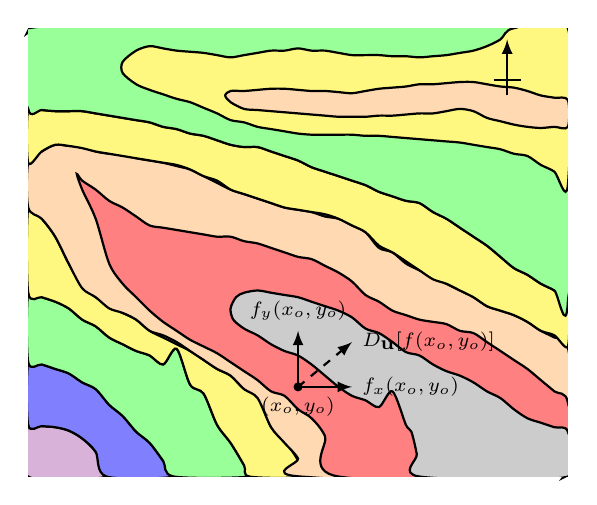
\begin{tikzpicture}
        \begin{axis}[xmin = 0, xmax = 20, ymin = 0, ymax = 20, ticks = none, 
        axis lines = center]
        \draw[fill = violet!30, draw = black, thick] plot[smooth cycle] 
        coordinates {(0, 2.3) (0.5, 2.25) (1, 2.2) (1.5, 2.05) (2, 1.7) 
        (2.5, 1.1) (2.9, 0) (0,0)};
        \draw[fill = blue!50, draw = black, thick] plot[smooth cycle] 
        coordinates {(0, 2.3) (0.5, 2.25) (1, 2.2) (1.5, 2.05) (2, 1.7) 
        (2.5, 1.1) (2.9, 0) (5.4, 0) (5, 0.7) (4.5, 1.5) (4, 2) (3.5, 2.7) 
        (3, 3.2) (2.5, 3.9) (2, 4.2) (1.5, 4.6) (1, 4.8) (0.5, 5) (0, 5.1)};
        \draw[fill = green!40, draw = black, thick] plot[smooth cycle] 
        coordinates {(5.4, 0) (5, 0.7) (4.5, 1.5) (4, 2) (3.5, 2.7) (3, 3.2) 
        (2.5, 3.9) (2, 4.2) (1.5, 4.6) (1, 4.8) (0.5, 5) (0, 5.1) (0, 8.2) 
        (0.5, 8) (1, 7.8) (1.5, 7.5) (2, 7) (2.5, 6.7) (3, 6.2) (3.5, 5.9) 
        (4, 5.6) (4.5, 5.4) (5, 5) (5.5, 5.7) (6, 4.1) (6.5, 3.7) (7, 2.3) 
        (7.5, 1.5) (8, 0.5) (8.2, 0)};
        \draw[fill = yellow!50, draw = black, thick] plot[smooth cycle] 
        coordinates {(0, 8.2) (0.5, 8) (1, 7.8) (1.5, 7.5) (2, 7) (2.5, 6.7) 
        (3, 6.2) (3.5, 5.9) (4, 5.6) (4.5, 5.4) (5, 5) (5.5, 5.7) (6, 4.1) 
        (6.5, 3.7) (7, 2.3) (7.5, 1.5) (8, 0.5) (8.2, 0) (10.1, 0) (10, 0.7) 
        (9.5, 1.6) (9, 2.2) (8.5, 3.6) (8, 3.9) (7.5, 4.5) (7, 4.8) (6.5, 5.2) 
        (6, 5.6) (5.5, 5.9) (5, 6.2) (4.5, 6.5) (4, 7) (3.5, 7.3) (3, 7.6) 
        (2.5, 8) (2, 8.5) (1.5, 9.5) (1, 10.7) (0.5, 11.5) (0, 12)};
        \draw[fill = orange!30, draw = black, thick] plot[smooth cycle] 
        coordinates {(20, 0) (10.1, 0) (10, 0.8) (9.5, 1.5) (9, 2.2) 
        (8.5, 3.5) (8, 3.9) (7.5, 4.5) (7, 4.8) (6.5, 5.2) (6, 5.6) (5.5, 6) 
        (5, 6.3) (4.5, 6.5) (4, 7) (3.5, 7.3) (3, 7.5) (2.5, 8) (2, 8.4) 
        (1.5, 9.5) (1, 10.7) (0.5, 11.5) (0, 12) (0, 14) (0.5, 14.5) (1, 14.8) 
        (1.5, 14.75) (2, 14.7) (2.5, 14.5) (3, 14.4) (3.5, 14.35) (4, 14.2) 
        (4.5, 14.1) (5, 14) (5.5, 13.85) (6, 13.7) (6.5, 13.4) (7, 13.1) 
        (7.5, 12.8) (8, 12.6) (8.5, 12.4) (9, 12.2) (9.5, 12) (10, 11.9) 
        (10.5, 11.8) (11, 11.6) (11.5, 11.5) (12, 11.2) (12.5, 10.9) 
        (13, 10.2) (13.5, 10) (14, 9.5) (14.5, 9.2) (15, 8.9) (15.5, 8.6) 
        (16, 8.3) (16.5, 8) (17, 7.6) (17.5, 7.4) (18, 7.2) (18.5, 6.9) 
        (19, 6.5) (19.5, 6.2) (20, 5.8)};
        \draw[fill = red!50, draw = black, thick] plot[smooth cycle] 
        coordinates {(20, 0) (11.5, 0) (11, 1.8) (10.5, 2.6) (10, 3) 
        (9.5, 3.6) (9, 3.8) (8.5, 4.3) (8, 4.7) (7.5, 5.1) (7, 5.5) (6.5, 5.8) 
        (6, 6.1) (5.5, 6.5) (5, 6.9) (4.5, 7.4) (4, 8) (3.5, 8.6) (3, 9.5) 
        (2.5, 11.5) (2, 12.8) (1.8, 13.5) (2, 13.2) (2.5, 12.8) (3, 12.3) 
        (3.5, 12) (4, 11.6) (4.5, 11.2) (5, 11.1) (5.5, 11) (6, 10.9) 
        (6.5, 10.8) (7, 10.7) (7.5, 10.7) (8, 10.5) (8.5, 10.4) (9, 10.2) 
        (9.5, 10) (10, 9.8) (10.5, 9.7) (11, 9.4) (11.5, 9.1) (12, 8.7) 
        (12.5, 8.1) (13, 7.8) (13.5, 7.4) (14, 7.2) (14.5, 7) (15, 6.9) 
        (15.5, 6.8) (16, 6.5) (16.5, 6.4) (17, 6) (17.5, 5.6) (18, 5.2) 
        (18.5, 4.8) (19, 4.3) (19.5, 3.8) (20, 3.3)};
        \draw[fill = gray!40, draw = black, thick] plot[smooth cycle] 
        coordinates {(14.5, 0) (14.4, 1) (14.2, 2) (14, 2.3) (13.5, 3.8) 
        (13, 3.1) (12.5, 3.4) (12, 3.6) (11.5, 4) (11, 4.5) (10.5, 5) 
        (10, 5.4) (9.5, 5.6) (9, 5.9) (8.5, 6.3) (8, 6.6) (7.6, 7) (7.5, 7.5) 
        (7.7, 8) (8, 8.2) (8.5, 8.3) (9, 8.2) (9.5, 8.1) (10, 8) (10.5, 7.8) 
        (11, 7.6) (11.5, 7.4) (12, 7.1) (12.5, 6.6) (13, 6.4) (13.5, 6) 
        (14, 5.55) (14.5, 5.4) (15, 5) (15.5, 4.7) (16, 4.5) (16.5, 4.2) 
        (17, 3.8) (17.5, 3.5) (18, 3) (18.5, 2.6) (19, 2.4) (19.5, 2.2) 
        (20, 2) (20, 0)};
        \draw[fill = yellow!50, draw = black, thick] plot[smooth cycle] 
        coordinates {(0, 14) (0.5, 14.5) (1, 14.8) (1.5, 14.75) (2, 14.65) 
        (2.5, 14.5) (3, 14.4) (3.5, 14.3) (4, 14.2) (4.5, 14.1) (5, 14) 
        (5.5, 13.9) (6, 13.7) (6.5, 13.4) (7, 13.2) (7.5, 12.8) (8, 12.6) 
        (8.5, 12.4) (9, 12.2) (9.5, 12) (10, 11.9) (10.5, 11.8) (11, 11.7) 
        (11.5, 11.5) (12, 11.2) (12.5, 10.9) (13, 10.3) (13.5, 10) (14, 9.6) 
        (14.5, 9.2) (15, 8.8) (15.5, 8.6) (16, 8.3) (16.5, 8) (17, 7.6) 
        (17.5, 7.4) (18, 7.2) (18.5, 6.9) (19, 6.5) (19.5, 6.3) (20, 5.8) 
        (20, 7.8) (19.5, 8.3) (19, 8.6) (18.5, 9) (18, 9.3) (17.5, 9.8) 
        (17, 10.3) (16.5, 10.7) (16, 11.1) (15.5, 11.5) (15, 11.8) 
        (14.5, 12.2) (14, 12.3) (13.5, 12.5) (13, 12.7) (12.5, 13) (12, 13.2) 
        (11.5, 13.4) (11, 13.6) (10.5, 13.8) (10, 14.1) (9.5, 14.3) (9, 14.5) 
        (8.5, 14.7) (8, 14.7) (7.5, 14.8) (7, 15) (6.5, 15.2) (6, 15.3) 
        (5.5, 15.5) (5, 15.6) (4.5, 15.8) (4, 15.9) (3.5, 16) (3, 16.1) 
        (2.5, 16.2) (2, 16.3) (1.5, 16.3) (1, 16.3) (0.5, 16.35) (0, 16.4)};
        \draw[fill = green!40, draw = black, thick] plot[smooth cycle] 
        coordinates {(20, 7.8) (19.5, 8.3) (19, 8.6) (18.5, 9) (18, 9.3) 
        (17.5, 9.8) (17, 10.3) (16.5, 10.7) (16, 11.1) (15.5, 11.5) (15, 11.8) 
        (14.5, 12.2) (14, 12.3) (13.5, 12.5) (13, 12.7) (12.5, 13) (12, 13.2) 
        (11.5, 13.4) (11, 13.6) (10.5, 13.8) (10, 14.1) (9.5, 14.3) (9, 14.5) 
        (8.5, 14.7) (8, 14.7) (7.5, 14.8) (7, 15) (6.5, 15.2) (6, 15.3) 
        (5.5, 15.5) (5, 15.6) (4.5, 15.8) (4, 15.9) (3.5, 16) (3, 16.1) 
        (2.5, 16.2) (2, 16.3) (1.5, 16.3) (1, 16.3) (0.5, 16.35) (0, 16.4) 
        (0, 20) (20, 20)};
        \draw[fill = yellow!50, draw = black, thick] plot[smooth cycle] 
        coordinates {(20, 13) (19.5, 13.6) (19, 13.9) (18.5, 14.3) (18, 14.4) 
        (17.5, 14.6) (17, 14.7) (16.5, 14.8) (16, 14.9) (15.5, 14.95) (15, 15) 
        (14.5, 15.05) (14, 15.1) (13.5, 15.15) (13, 15.2) (12.5, 15.2) 
        (12, 15.25) (11.5, 15.25) (11, 15.25) (10.5, 15.25) (10, 15.3) 
        (9.5, 15.4) (9, 15.5) (8.5, 15.6) (8, 15.8) (7.5, 15.9) (7, 16.2) 
        (6.5, 16.45) (6, 16.7) (5.5, 16.85) (5, 17.05) (4.5, 17.25) (4, 17.5) 
        (3.5, 18) (3.5, 18.5) (4, 19) (4.5, 19.2) (5, 19.1) (5.5, 19) 
        (6, 18.95) (6.5, 18.9) (7, 18.8) (7.5, 18.7) (8, 18.8) (8.5, 18.9) 
        (9, 19) (9.5, 19) (10, 19.1) (10.5, 19) (11, 19) (11.5, 18.9) 
        (12, 18.8) (12.5, 18.8) (13, 18.8) (13.5, 18.75) (14, 18.75) 
        (14.5, 18.7) (15, 18.75) (15.5, 18.8) (16, 18.9) (16.5, 19) (17, 19.2) 
        (17.5, 19.5) (18, 20) (20, 20)};
        \draw[fill = orange!30, draw = black, thick] plot[smooth cycle] 
        coordinates {(20, 15.6) (19.5, 15.6) (19, 15.55) (18.5, 15.6) 
        (18, 15.7) (17.5, 15.85) (17, 16) (16.5, 16.3) (16, 16.4) (15.5, 16.3) 
        (15, 16.2) (14.5, 16.2) (14, 16.15) (13.5, 16.1) (13, 16.1) 
        (12.5, 16.05) (12, 16.05) (11.5, 16.05) (11, 16.1) (10.5, 16.15) 
        (10, 16.2) (9.5, 16.25) (9, 16.3) (8.5, 16.35) (8, 16.4) (7.5, 16.7) 
        (7.3, 17) (7.5, 17.2) (8, 17.2) (8.5, 17.25) (9, 17.3) (9.5, 17.3) 
        (10, 17.25) (10.5, 17.2) (11, 17.2) (11.5, 17.15) (12, 17.1) 
        (12.5, 17.2) (13, 17.3) (13.5, 17.35) (14, 17.4) (14.5, 17.5) 
        (15, 17.5) (15.5, 17.55) (16, 17.6) (16.5, 17.6) (17, 17.5) 
        (17.5, 17.4) (18, 17.35) (18.5, 17.2) (19, 17) (19.5, 16.9) 
        (20, 16.8)};
        \draw[black, fill = black] (10, 4) circle (0.5mm) node[below, 
        font = \scriptsize] {$(x_o, y_o)$};
        \draw[black, thick, -latex] (10, 4) -- (10, 6.5) node[above, 
        font = \scriptsize] {$f_y(x_o, y_o)$}; 
        \draw[black, thick, -latex] (10, 4) -- (12, 4) node[right, 
        font = \scriptsize] {$f_x(x_o, y_o)$};
        \draw[black, thick, dashed, -latex] (10, 4) -- (12, 6) node[right, 
        font = \scriptsize] {$D_{\textbf{u}} [f(x_o, y_o)]$};
        \draw[-latex, black, thick] (17.75, 17) -- (17.75, 19.5);
        \draw[black, thick] (17.25, 17.7) -- (18.25, 17.7);
        \end{axis}
    \end{tikzpicture}
    \caption{If \textbf{u} points north-east, then the directional derivative 
    of $f(x, y)$ at $(x_o, y_o)$, $D_{\textbf{u}} \left[ f(x_o, y_o ) 
    \right]$, tells the rate of change going north-east}
    \label{fig:mount_deriv}
\end{figure}

To find the rate of change at $(x_o, y_o)$, in the direction of some arbitrary 
unit vector, $\textbf{u} = \left[ a, b \right] = a\textbf{i} + b\textbf{j}$, 
we first note that the point $Q = (x_o, y_o, z_o)$, where $z_o = f(x_o, y_o)$, 
lies on the surface defined by $z = f(x, y)$. There is a vertical plane, $P$, 
that passes through $Q$ and points in the direction of \textbf{u}. This 
intersection defines curve $C$, which lies on the surface, and the slope of 
this curve at $Q = (x_o, y_o, z_o)$ is the directional derivative of $f$ in 
the direction of \textbf{u} (see figure \ref{fig:direct_deriv}). 

\begin{figure}[H]
    \centering
    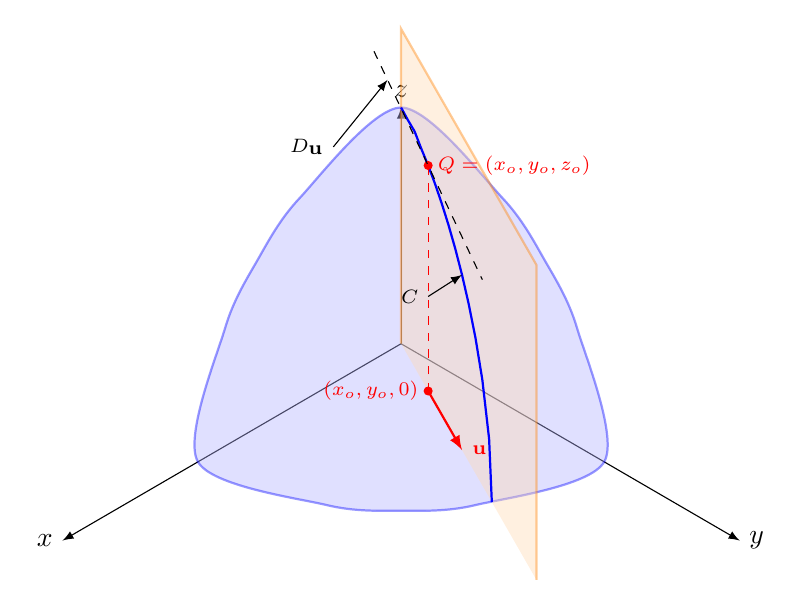
\begin{tikzpicture}[x = {(-0.86cm, -0.5cm)}, y = {(0.86cm, -0.5cm)}, 
    z = {(0cm, 1cm)}]
        \draw[-latex] (0,0,0) -- (5,0,0) node[left] {$x$};
        \draw[-latex] (0,0,0) -- (0,5,0) node[right] {$y$};
        \draw[-latex] (0,0,0) -- (0,0,3) node[above] {$z$};
        \draw[blue, thick, fill = blue!30, opacity = 0.4] plot[smooth cycle] 
        coordinates {(3, 0, 0) (2.598, 0, 1.5) (2.121, 0, 2.121) 
        (1.5, 0, 2.598) (0, 0, 3) (0, 1.5, 2.598) (0, 2.121, 2.121) 
        (0, 2.598, 1.5) (0, 3, 0) (1.5, 2.598, 0) (2.121, 2.121, 0) 
        (2.598, 1.5, 0)};
        \draw[orange, thick, fill = orange!30, opacity = 0.4] (0, 0, 0) -- 
        (0, 0, 4) -- (2, 4, 4) -- (2, 4, 0);
        \draw[red, thick, -latex] (0.4, 0.8, 0) -- (0.9, 1.8, 0) 
        node[right, font = \scriptsize] {\textbf{u}};
        \draw[blue, thick] (0,0,3) -- (0.1, 0.2, 2.992) -- (0.2, 0.4, 2.996) 
        -- (0.3, 0.6, 2.924) -- (0.4, 0.8, 2.864) -- (0.5, 1, 2.784) -- 
        (0.6, 1.2, 2.683) -- (0.7, 1.4, 2.559) -- (0.8, 1.6, 2.408) -- 
        (0.9, 1.8, 2.225) -- (1, 2, 2) -- (1.1, 2.2, 1.718) -- 
        (1.2, 2.4, 1.342) -- (1.3, 2.6, 0.742) -- (1.34, 2.68, 0);
        \draw[latex-] (0.9, 1.8, 2.225) -- (1.2, 1.6, 2) 
        node[left, font = \scriptsize] {$C$};
        \draw[red, dashed] (0.4, 0.8, 0) -- (0.4, 0.8, 2.864);
        \draw[red, fill = red] (0.4, 0.8, 2.864) circle (0.5mm) 
        node[right, font = \scriptsize] {$Q = (x_o, y_o, z_o)$};
        \draw[red, fill = red] (0.4, 0.8, 0) circle (0.5mm) 
        node[left, font = \scriptsize] {$(x_o, y_o, 0)$};
        \draw[black, dashed] (-0.4, -0.8, 3.11384) -- (1.2, 2.4, 2.6142);
        \draw[latex-] (-0.2, -0.4, 3.0514) -- (1, 0, 3) 
        node[left, font = \scriptsize] {$D_{\textbf{u}}$}; 
    \end{tikzpicture}
    \caption{The slope of the curve formed between the plane parallel to 
    \textbf{u} and the surface $z = f(x, y)$ is the directional derivative, 
    $D_{\textbf{u}}$}
    \label{fig:direct_deriv}
\end{figure}

We can choose another point, $R = (x, y, z)$, that is $h$ units away from $Q$ 
along \textbf{u} (see \ref{fig:direct_deriv2}). Then the change in $x$ is $x - 
x_o = ha$ and the change in $y$ is $y - y_o = hb$. And the slope from $Q$ to 
$R$ is given by:
$$\frac{\Delta z}{h} = \frac{f(x, y) - f(x_o, y_o)}{h}$$

\begin{figure}[H]
    \centering
    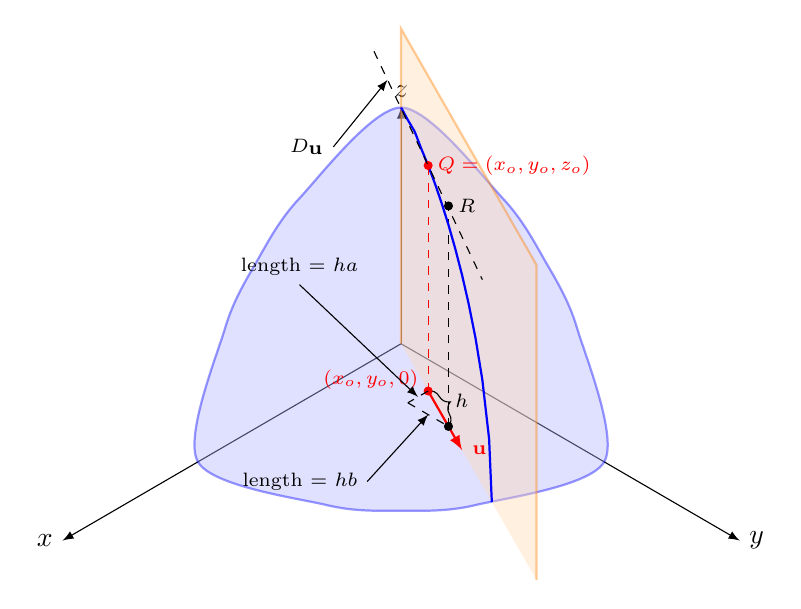
\begin{tikzpicture}[x = {(-0.86cm, -0.5cm)}, y = {(0.86cm, -0.5cm)}, 
    z = {(0cm, 1cm)}]
        \draw[-latex] (0,0,0) -- (5,0,0) node[left] {$x$};
        \draw[-latex] (0,0,0) -- (0,5,0) node[right] {$y$};
        \draw[-latex] (0,0,0) -- (0,0,3) node[above] {$z$};
        \draw[blue, thick, fill = blue!30, opacity = 0.4] plot[smooth cycle] 
        coordinates {(3, 0, 0) (2.598, 0, 1.5) (2.121, 0, 2.121) 
        (1.5, 0, 2.598) (0, 0, 3) (0, 1.5, 2.598) (0, 2.121, 2.121) 
        (0, 2.598, 1.5) (0, 3, 0) (1.5, 2.598, 0) (2.121, 2.121, 0) 
        (2.598, 1.5, 0)};
        \draw[orange, thick, fill = orange!30, opacity = 0.4] (0, 0, 0) -- 
        (0, 0, 4) -- (2, 4, 4) -- (2, 4, 0);
        \draw[red, thick, -latex] (0.4, 0.8, 0) -- (0.9, 1.8, 0) 
        node[right, font = \scriptsize] {\textbf{u}};
        \draw[black, fill = black] (0.7, 1.4, 0) circle (0.5mm);
        \draw[decorate, decoration = {brace, amplitude = 5pt}] (0.4, 0.8, 0) 
        -- (0.7, 1.4, 0) node[midway, xshift = 0.3cm, yshift = 0.1cm, 
        font = \scriptsize] {$h$};
        \draw[dashed] (0.7, 1.4, 0) -- (0.7, 1.4, 2.8);
        \draw[black, fill = black] (0.7, 1.4, 2.8) circle (0.5mm) node[right, 
        font = \scriptsize] {$R$};
        \draw[blue, thick] (0,0,3) -- (0.1, 0.2, 2.992) -- (0.2, 0.4, 2.996) 
        -- (0.3, 0.6, 2.924) -- (0.4, 0.8, 2.864) -- (0.5, 1, 2.784) -- 
        (0.6, 1.2, 2.683) -- (0.7, 1.4, 2.559) -- (0.8, 1.6, 2.408) -- 
        (0.9, 1.8, 2.225) -- (1, 2, 2) -- (1.1, 2.2, 1.718) -- 
        (1.2, 2.4, 1.342) -- (1.3, 2.6, 0.742) -- (1.34, 2.68, 0);
        \draw[red, dashed] (0.4, 0.8, 0) -- (0.4, 0.8, 2.864);
        \draw[red, fill = red] (0.4, 0.8, 2.864) circle (0.5mm) 
        node[right, font = \scriptsize] {$Q = (x_o, y_o, z_o)$};
        \draw[red, fill = red] (0.4, 0.8, 0) circle (0.5mm) 
        node[left, font = \scriptsize, yshift = 0.15cm] {$(x_o, y_o, 0)$};
        \draw[black, dashed] (-0.4, -0.8, 3.11384) -- (1.2, 2.4, 2.6142);
        \draw[latex-] (-0.2, -0.4, 3.0514) -- (1, 0, 3) 
        node[left, font = \scriptsize] {$D_{\textbf{u}}$}; 
        \draw[dashed] (0.4, 0.8, 0) -- (0.7, 0.8, 0);
        \draw[dashed] (0.7, 0.8, 0) -- (0.7, 1.4, 0);
        \draw[latex-] (0.7, 1.1, 0) -- (2, 1.5, 0) node[left, font = 
        \scriptsize] {length = $hb$};
        \draw[latex-] (0.55, 0.8, 0) -- (1.5, 0, 1.5) node[above, font = 
        \scriptsize] {length = $ha$};
    \end{tikzpicture}
    \caption{A second point, $R$, along \textbf{u} is $h$ units away along 
    \textbf{u}}
    \label{fig:direct_deriv2}
\end{figure}

We find the directional derivative by substituting for $x$ and $y$ and taking 
the limit as $h$ goes to zero:
$$D_{\textbf{u}} f(x_0, y_0) = \lim_{h \to 0} \frac{f(x_o + ha, y_o + hb) - 
f(x_o, y_o)}{h}$$

How is this related to $f_x$ and $f_y$? Let us define $g(h)$ such that $g(h) = 
f(x_o + ha, y_o + hb)$. Then
$$g'(0) = \lim_{h \to 0} \frac{g(h) - g(0)}{h}$$
$$= \lim_{h \to 0} \frac{f(x_o + ha, y_o + hb) - f(x_o, y_o)}{h} = 
D_{\textbf{u}} f(x_o, y_o)$$

We can also apply the Chain Rule to $g(h)$:
$$g'(h) = \frac{\partial f}{\partial x} \frac{dx}{dh} + \frac{\partial f}{
\partial y} \frac{dy}{dh} = f_x(x, y)a + f_y(x, y)b$$

Substituting $h = 0$, $x = x_o$, and $y = y_o$, we see that:
$$g'(0) = f_x(x_o, y_o)a + f_y(x_o, y_o)b$$

Which means that:
$$D_{\textbf{u}} f(x_o, y_o) = f_x(x_o, y_o)a + f_y(x_o, y_o)b$$

So a directional derivative is:

\begin{mdframed}[style = important, frametitle = {The Directional Derivative}]
Let $f$ be a differentiable function and \textbf{u} be a unit vector, 
$\textbf{u} = \left[ a, b \right]$. Then the directional derivative in the 
direction of \textbf{u} is:
\begin{equation}
    D_{\textbf{u}} f(x, y) = f_x(x, y)a + f_y(x, y)b = \textbf{u}_x \left[ 
    \frac{\partial}{\partial x} f(x, y) \right] + \textbf{u}_y \left[ \frac{
    \partial}{\partial y} f(x, y) \right]
    \label{eq:directionalDeriv}
\end{equation}

Where $\textbf{u}_x$ and $\textbf{u}_y$ are the $x$- and $y$-components of 
\textbf{u}, respectively. 
\end{mdframed}


\textbf{Example}: Find the directional derivative $D_{\textbf{u}} f(x, y)$ if 
$f(x, y) = y^3 - 3xy + 4x^2$ and \textbf{u} is the unit vector given by the 
angle $\theta = \pi/3$. What is the rate of change in the direction of 
\textbf{u} at $(1, 2)$?

\textbf{Solution}: We can describe \textbf{u} thusly:
$$\textbf{u} = \left[ \cos{ \frac{\pi}{3} }, \sin{ \frac{\pi}{3}} \right] = 
\left[ \frac{1}{2}, \frac{\sqrt{3}}{2} \right]$$

And therefore:
$$D_{\textbf{u}} f(x, y) = f_x(x, y) \left( \frac{1}{2} \right) + f_y(x, y) 
\left( \frac{\sqrt{3}}{2} \right) $$
$$= \frac{\partial}{\partial x} \left( y^3 - 3xy + 4x^2 \right) \left( 
\frac{1}{2} \right) + \frac{\partial}{\partial y} \left( y^3 - 3xy + 4x^2 
\right) \left( \frac{\sqrt{3}}{2} \right)$$
$$= \frac{1}{2} \left( -3y + 8x \right) + \frac{\sqrt{3}}{2} \left( 3y^2 - 3x 
\right)$$
$$= \frac{-3}{2}y + 4x + \frac{3\sqrt{3}}{2}y^2 - \frac{3\sqrt{3}}{2}x = \frac{
3\sqrt{3}}{2}y^2 + \frac{8-3\sqrt{3}}{2}x - \frac{3}{2}y$$

And therefore $D_{\textbf{u}} f(1, 2)$ is:
$$= \frac{3\sqrt{3}}{2} \left( 2 \right)^2 + \frac{8 - 3\sqrt{3}}{2} \left( 1 
\right) - \frac{3}{2} \left( 2 \right) = 6\sqrt{3} + 4 - \frac{3\sqrt{3}}{2} - 
3$$
$$= 1 + \frac{9\sqrt{3}}{2}$$

\subsection{Unit Vectors in Two Dimensions}\index{unit vector}

What if the given vector is not a unit vector? We can scale the given vector 
to find a unit vector in the same direction:

\textbf{Example}: Find the directional derivative of $f(x, y) = 3x\sqrt{y}$ 
at $(1, 4)$ in the direction of $\textbf{v} = \left[2, 1 \right]$.

\textbf{Solution}: First, we need to find a unit vector in the same direction 
as \textbf{v}. There are several ways to do this. In two dimensions, a unit 
vector in the same direction as \textbf{v} can be found using trigonometry 
(see figure \ref{fig:vector} for an illustration). 

\begin{figure}[H]
    \centering
    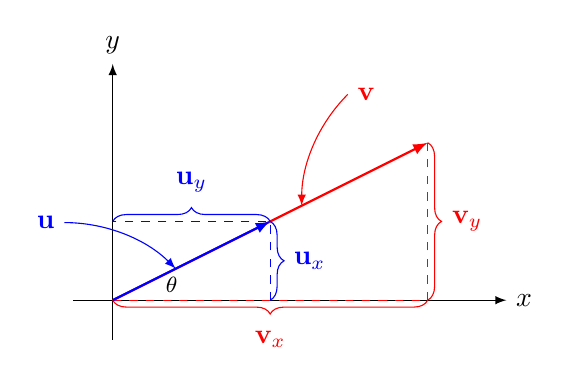
\begin{tikzpicture}
        \draw[black, -latex] (-0.5, 0) -- (5, 0) node[right] {$x$};
        \draw[black, -latex] (0, -0.5) -- (0, 3) node[above] {$y$};
        \draw[red, thick, -latex] (0, 0) -- (4, 2);
        \draw[red, thin, dashed] (0,0) -- (4, 0);
        \draw[red, thin, dashed] (4, 0) -- (4, 2);
        \draw[red, decorate, decoration = {brace, amplitude = 5pt, mirror}] 
        (0, 0) -- (4, 0) node[midway, yshift = -0.5cm] {$\textbf{v}_x$};
        \draw[red, decorate, decoration = {brace, amplitude = 5pt, mirror}] 
        (4, 0) -- (4, 2) node[midway, xshift = 0.5cm] {$\textbf{v}_y$};
        \draw[red, latex-] (2.4, 1.2) arc(180:135:2) node[right] {\textbf{v}};
        \draw[blue, thick, -latex] (0, 0) -- (2, 1);
        \draw[blue, latex-] (0.8, 0.4) arc(45:90:2) node[left] {\textbf{u}};
        \node[font = \footnotesize] at (0.75, 0.2) {$\theta$};
        \draw[blue, thin, dashed] (2, 0) -- (2, 1) -- (0, 1);
        \draw[blue, decorate, decoration = {brace, amplitude = 5pt, mirror}] 
        (2, 0) -- (2, 1) node[midway, xshift = 0.5cm] {$\textbf{u}_x$};
        \draw[blue, decorate, decoration = {brace, amplitude = 5pt}] 
        (0, 1) -- (2, 1) node[midway, yshift = 0.5cm] {$\textbf{u}_y$};
    \end{tikzpicture}
    \caption{\textbf{u} is a unit vector in the same direction as \textbf{v}}
    \label{fig:vector}
\end{figure}

We know that $\theta = \arctan{ \left( \textbf{v}_y / \textbf{v}_x \right)}$. 
Therefore, the $x$-component of the unit vector, \textbf{u}, is given by:
$$\textbf{u}_x = |\textbf{u}| \cos{ \theta} = \cos{ \left( \arctan{ \frac{
\textbf{v}_y}{\textbf{v}_x}} \right)}$$

Similarly, we know that:
$$\textbf{u}_y = |\textbf{u}| \sin{ \theta} = \sin{ \left( \arctan{ \frac{
\textbf{v}_y}{\textbf{v}_x}} \right)}$$

(Recall that since \textbf{u} is a unit vector, $|\textbf{u}| = 1$). 

Let us use this method to find a unit vector, \textbf{u}, in the same direction 
as $\textbf{v} = \left[ 2, 1 \right]$:
$$\textbf{u}_x = \cos{ \left( \arctan{ \frac{1}{2} } \right) } \approx \cos{ 
\left( 0.464 \right) } = \frac{2}{\sqrt{5}}$$
$$\textbf{u}_y = \sin{ \left( \arctan{ \frac{1}{2} } \right) } \approx \sin{ 
\left( 0.464 \right)} = \frac{1}{\sqrt{5}}$$

Therefore, a unit vector in the same direction as \textbf{v} is $\textbf{u} = 
\left[ 2/\sqrt{5}, 1/\sqrt{5} \right]$. 

And we can find the directional derivative:
$$D_{\textbf{u}}(x, y) = \textbf{u}_x \left[ \frac{\partial}{\partial x} f(x, 
y) \right] + \textbf{u}_y \left[ \frac{\partial}{\partial y} f(x, y) \right]$$
$$D_{\textbf{u}}(x, y) = \left( \frac{2}{\sqrt{5}} \right) \left[ \frac{
\partial}{\partial x} \left( 3x\sqrt{y} \right) \right] + \left( \frac{1}{
\sqrt{5}} \right) \left[ \frac{\partial}{\partial y} \left( 3x\sqrt{y} \right) 
\right]$$
$$D_{\textbf{u}}(x, y) = \left( \frac{2}{\sqrt{5}} \right) \left( 3\sqrt{y} 
\right) + \left( \frac{1}{\sqrt{5}} \right) \left( \frac{3x}{2\sqrt{y}} 
\right)$$
$$D_{\textbf{u}}(x, y) = \frac{12y + 3x}{2\sqrt{5y}}$$

To find the value of the directional derivative at $(1, 4)$, we 
substitute for $x$ and $y$:
$$D_{\textbf{u}}(1, 4) = \frac{12(4) + 3(1)}{2\sqrt{5(4)}} = \frac{51}{4\sqrt{5}} 
\approx 5.702$$

\subsection{Unit Vectors in Higher Dimensions}
The trigonometric explanation for finding unit vectors is more difficult to 
visualize in higher dimensions. However, there is another method that works 
well in 2, 3, and higher dimensions. Recall that the magnitude of a vector, 
$\textbf{v} = \left[ \textbf{v}_x, \textbf{v}_y \right]$ is given by $| 
\textbf{v} | = \sqrt{\left( \textbf{v}_x \right)^2 + \left( \textbf{v}_y 
\right)^2}$. For a vector with $n$ dimensions, $\textbf{v} = \left[ \textbf{v}_
1, \textbf{v}_2, \cdots , \textbf{v}_n \right]$, the magnitude is given by $| 
\textbf{v} | = \sqrt{ \left( \textbf{v}_1 \right)^2 + \left( \textbf{v}_2 
\right)^2 + \cdots + \left( \textbf{v}_n \right)^2}$. 

To find a unit vector, \textbf{u}, in the same direction as \textbf{v}, we can 
scale \textbf{v} up or down so that its magnitude is 1. We can do this by 
dividing by \textbf{v}'s magnitude. Consider the two-dimensional vector used 
in the last example, $\textbf{v} = \left[ 2, 1 \right]$. Its magnitude is:
$$| \textbf{v} | = \sqrt{\left( 2 \right)^2 + \left( 1 \right)^2} = \sqrt{5}$$

Let us check if $\textbf{v} / | \textbf{v} |$ is a unit vector:
$$ \frac{\textbf{v}}{|\textbf{v}|} = \left( \frac{1}{\sqrt{5}} \right) \left[ 
2, 1 \right] = \left[ \frac{2}{\sqrt{5}}, \frac{1}{\sqrt{5}} \right]$$

And the magnitude of this scaled vector is:
$$ \left| \frac{\textbf{v}}{| \textbf{v} |} \right| = \sqrt{\left( \frac{2}{
\sqrt{5}} \right)^2 + \left( \frac{1}{\sqrt{5}} \right)^2} = \sqrt{\frac{4}{5} 
+ \frac{1}{5}} = \sqrt{1} = 1$$

Notice our unit vector is the same as we found using the trigonometric method 
above. 

Another way to think of the question is: what factor, $k$, can we multiply 
\textbf{v} by to yield a vector with a magnitude of 1? Let us see this method 
for the 3-dimensional vector $\textbf{v} = \left[ 3, 2, 1 \right]$. We are 
looking for a $k$ such that:
$$|k\textbf{v}| = 1$$
$$|k \textbf{v}| = \left| \left[ 3k, 2k, 1k \right] \right| = \sqrt{\left( 3k 
\right)^2 + \left( 2k \right)^2 + \left( 1k \right)^2}$$
$$= \sqrt{9k^2 + 4k^2 + k^2} = k\sqrt{14} = 1$$

Which implies that $k = 1/\sqrt{14}$, which is $1/|\textbf{v}|$. And therefore 
a unit vector in the same direction as $\textbf{v} = \left[ 3, 2, 1 \right]$ 
is:
$$\textbf{u} = \frac{1}{\sqrt{14}} \left[ 3, 2, 1 \right] = \left[ \frac{3}{
\sqrt{14}}, \frac{2}{\sqrt{14}}, \frac{1}{\sqrt{14}} \right]$$


\begin{Exercise}[title = {Finding Directional Derivatives}, label = direction]
Find the directional derivative of the function at the given point in the 
direction of the given vector. 
\begin{enumerate}
    \item $f(x, y) = e^{3x} \sin{2y}$, $(0, \pi/6)$, $\textbf{v} = \left[ -3, 
    4 \right]$
    \item $f(x, y) = x^2y + xy^3$, $(2, 4)$, $\textbf{v} = 2 \textbf{i} - 
    \textbf{j}$
    \item $f(x, y, z) = \ln{ \left( x^2 + 3y - z \right)}$, $(2, 2, 1)$, 
    $\textbf{v} = \left[ 1, 1, 1 \right]$
\end{enumerate}
\end{Exercise}

\begin{Answer}[ref = direction]
\begin{enumerate}
    \item First, we define \textbf{u} such that $|\textbf{u}| = 1$ and 
    \textbf{u} is in the same direction as \textbf{v}:
    $$\textbf{u} = k \textbf{v} = \left[ -3k, 4k \right]$$
    $$\sqrt{ \left( -3k \right)^2 + \left( 4k \right)^2} = 1$$
    $$\sqrt{9k^2 + 16k^2} = \sqrt{25k^2} = 5k = 1$$
    $$k = \frac{1}{5}$$

    Therefore, we define $\textbf{u} = \left[ -3/5, 4/5 \right]$ and the 
    directional derivative is given by:
    $$D_u(x, y) = \left( \frac{-3}{5} \right) \frac{\partial}{\partial x} f(x, 
    y) + \left( \frac{4}{5} \right) \frac{\partial}{\partial y} f(x, y)$$
    $$= \left( \frac{-3}{5} \right) \frac{\partial}{\partial x} \left[ e^{3x} 
    \sin{2y} \right] + \left( \frac{4}{5} \right) \frac{\partial}{\partial y} 
    \left[ e^{3x} \sin{2y} \right]$$
    $$= \left( \frac{-3}{5} \right) \left( 3e^{3x} \sin{2y} \right) + \left( 
    \frac{4}{5} \right) \left( 2e^{3x} \cos{2y} \right)$$

    And substituting for $(x, y) = (0, \pi/6)$:
    $$D_u(0, \pi/6) = \left( \frac{-3}{5} \right) \cdot \left[ 3e^{3 \cdot 0} 
    \sin{ \left( \frac{\pi}{3} \right)} \right] + \left( \frac{4}{5} \right) 
    \cdot \left[ 2e^{3 \cdot 0} \cos{ \left( \frac{\pi}{3} \right)} \right]$$
    $$D_u(0, \pi/6) = \left( \frac{-3}{5} \right) \cdot \left[ 3 \cdot \frac{
    \sqrt{3}}{2} \right] + \left( \frac{4}{5} \right) \cdot \left[ 2 \cdot 
    \frac{1}{2} \right]$$
    $$D_u(0, \pi/6) = \left( \frac{-3}{5} \right) \cdot \left( \frac{3
    \sqrt{3}}{2} \right) + \left( \frac{4}{5} \right) \cdot \left( 1 \right)$$
    $$D_u(0, \pi/6) = \frac{-9\sqrt{3}}{10} + \frac{8}{10} = \frac{8-9\sqrt{3}
    }{10} \approx -0.759$$

    \item We can express \textbf{v} as $\textbf{v} = \left[ 2, -1 \right]$. 
    And we define \textbf{u} such that $| \textbf{u} | = 1$ and \textbf{u} is 
    in the same direction as \textbf{v}:
    $$\textbf{u} = k\textbf{v} = \left[ 2k, -k \right]$$
    $$\sqrt{\left( 2k \right)^2 + \left( -k \right)^2} = 1$$
    $$\sqrt{4k^2 + k^2} = \sqrt{5}k = 1$$
    $$k = \frac{1}{\sqrt{5}} = \frac{\sqrt{5}}{5}$$

    Therefore, we define $\textbf{u} = \left[ 2\sqrt{5}/5, -\sqrt{5}/5 \right]$
    and the directional derivative is given by:
    $$D_u(x, y) = \left( \frac{2\sqrt{5}}{5} \right) \frac{\partial}{\partial 
    x}f(x, y) + \left( \frac{-\sqrt{5}}{5} \right) \frac{\partial}{\partial y}
    f(x, y)$$
    $$= \left( \frac{2\sqrt{5}}{5} \right) \frac{\partial}{\partial x} \left[ 
    x^2y + xy^3 \right] + \left( \frac{-\sqrt{5}}{5} \right) \frac{\partial}{
    \partial y} \left[ x^2y + xy^3 \right]$$
    $$= \left( \frac{2\sqrt{5}}{5} \right) \left[ 2xy + y^3 \right] + \left( 
    \frac{-\sqrt{5}}{5} \right) \left[ x^2 + 3xy^2 \right]$$

    And substituting $(x, y) = (2, 4)$:
    $$D_u(2, 4) = \left( \frac{2\sqrt{5}}{5} \right) \left[ 2(2)(4) + 4^3 
    \right] + \left( \frac{-\sqrt{5}}{5} \right) \left[ 2^2 + 3(2)(4^2) 
    \right]$$
    $$D_u(2, 4) = \left( \frac{2\sqrt{5}}{5} \right) \left[ 80 \right] + \left(
    \frac{-\sqrt{5}}{5} \right) \left[ 100 \right]$$
    $$D_u(2, 4) = 32\sqrt{5} - 20\sqrt{5} = 12\sqrt{5} \approx 26.833$$

    \item We define \textbf{u} such that $| \textbf{u} | = 1$ and \textbf{u} 
    is in the same direction as \textbf{v}:
    $$\textbf{u} = k\textbf{v} = \left[k, k, k \right]$$
    $$\sqrt{k^2 + k^2 + k^2} = 1$$
    $$\sqrt{3}k = 1$$
    $$k = \frac{1}{\sqrt{3}} = \frac{\sqrt{3}}{3}$$

    Therefore, we let $\textbf{u} = \left[ \sqrt{3}/3, \sqrt{3}/3, \sqrt{3}/3 
    \right]$ and the directional derivative is given by:
    $$D_u(x, y, z) = \left( \frac{\sqrt{3}}{3} \right) \frac{\partial}{
    \partial x} f(x, y, z) + \left( \frac{\sqrt{3}}{3} \right) \frac{
    \partial}{\partial y}f(x, y, z) + \left( \frac{\sqrt{3}}{3} \right) 
    \frac{\partial}{\partial z} f(x, y, z)$$
    $$= \left( \frac{\sqrt{3}}{3} \right) \left[ \frac{\partial}{\partial x} 
    \ln{ \left( x^2 + 3y - z \right)} + \frac{\partial}{\partial y} \ln{ 
    \left( x^2 + 3y - z \right)} + \frac{\partial}{\partial z} \ln{ \left( 
    x^2 + 3y - z \right)} \right]$$
    $$= \left( \frac{\sqrt{3}}{3} \right) \left[ \frac{2x}{x^2 + 3y - z} + 
    \frac{3}{x^2 + 3y - z} + \frac{-1}{x^2 + 3y - z} \right]$$
    $$= \left( \frac{\sqrt{3}}{3} \right) \left[ \frac{2x + 2}{x^2 + 3y - z} 
    \right] = \frac{\sqrt{3} \left( 2x + 2 \right)}{3 \left( x^2 + 3y - z 
    \right)}$$

    And substituting $(x, y, z) = (2, 2, 1)$:
    $$D_u(2, 2, 1) = \frac{\sqrt{3} \left( 2(2) + 2 \right)}{3 \left( 2^2 + 
    3(2) - 1 \right)} = \frac{\sqrt{3} \left( 6 \right)}{3 \left( 9 \right)} 
    = \frac{2\sqrt{3}}{9} \approx 0.385$$
\end{enumerate}
\end{Answer}

\subsection{The Direction of Steepest Ascent}\index{maximum rate of change}
The directional derivative can be written as the dot product of two vectors:
$$D_u f(x, y) = af_x(x, y) + bf_y(x, y) = \left[ f_x(x, y), f_y(x, y) \right] 
\cdot \textbf{u}$$

The first vector, $\left[ f_x(x, y), f_y(x, y) \right]$, is called \textit{the 
gradient of f}\index{gradient}, and is noted as $\nabla f$. 

\begin{mdframed}[style = important, frametitle = {The Gradient}]
For a two-variable function, $f(x, y)$, the gradient of $f$ is the vector:
$$\nabla f = \left[ f_x(x, y), f_y(x, y) \right] = \frac{\partial f}{\partial 
x} \textbf{i} + \frac{\partial f}{\partial y} \textbf{j}$$

Where \textbf{i} and \textbf{j} are the unit vectors in the $x$- and 
$y$-directions, respectively.
\end{mdframed}

Think back to the elevation example we opened the chapter with. What if we 
wanted to complete our ascent as quickly as possible? We would want to 
know the direction in which the elevation is changing the fastest. This occurs 
when the direction we are going is the same direction as the gradient vector, 
$\nabla f$. 

Recall that the dot product is defined as:
$$\textbf{u} \cdot \textbf{v} = \left| \textbf{u} \right| \left| \textbf{v} 
\right| \cos{ \theta}$$

Where $\theta$ is the angle between the vectors \textbf{u} and \textbf{v}. 
Applying this to the directional derivative, we see that:
$$D_u f = \nabla f \cdot \textbf{u} = \left| \nabla f \right| \left| 
\textbf{u} \right| \cos{\theta} = \left| \nabla f \right| \cos{\theta}$$

Which is at its maximum when $\nabla f$ and \textbf{u} point in the same 
direction (because $\cos{\left( 0 \right)} = 1$). Therefore, the gradient 
vector points in the direction of maximum change and the magnitude of that 
vector is the rate of maximum change. 

\textbf{Example}: Find the maximum rate of change of $f(x, y) = 4y\sqrt{x}$ at 
$(4, 1)$. In what direction does the maximum change occur?

\textbf{Solution}: We begin by finding $\nabla f$:
$$\nabla f = \left[ \frac{\partial}{\partial x} \left( 4y\sqrt{x} \right), 
\frac{\partial}{\partial y} \left( 4y\sqrt{x} \right) \right]$$
$$\nabla f = \left[ \frac{2y}{\sqrt{x}}, 4\sqrt{x} \right]$$

And thus, 
$$\nabla f(4, 1) = \left[ \frac{2(1)}{\sqrt{4}}, 4\sqrt{4} \right] = \left[ 1, 
8 \right]$$

Therefore, the maximum rate of change at $(4, 1)$ is:
$$\left| \nabla f \right| = \sqrt{1^2 + 8^2} = \sqrt{65}$$

in the direction of the vector $\left[ 1, 8 \right]$. 

\begin{Exercise}[title = {Using the Gradient to find Maximum Change}, 
label = maximum]
Suppose you are climbing a mountain whose elevation is described by $z = 3000 
- 0.01x^2 - 0.02y^2$. Take the positive $x$-direction to be east and the 
positive $y$-direction to be north. 
\begin{enumerate}
    \item If you are at $(x, y) = (50, 50)$, what is your elevation?
    \item If you walk south, will you ascend or descend?
    \item If you walk northwest, will you ascend or descend? Will the rate of 
    elevation change be greater or less than if you walked south?
    \item In what direction should you walk for the steepest ascent? What will 
    your ascension rate be?
\end{enumerate}
\end{Exercise}

\begin{Answer}[ref = maximum]
\begin{enumerate}
    \item $z = f(50, 50) = 3000 - 0.01(50)^2 - 0.02(50)^2 = 2925$
    \item A south-pointing unit vector is $\textbf{u} = \left[ 0, -1 \right]$. 
    To find the rate of change, we find the directional derivative in the 
    direction of \textbf{u} at $(50, 50)$:
    $$D_u f(x, y) = \left( -1 \right) \left[ \frac{\partial}{\partial y} 
    \left( 3000 - 0.01x^2 - 0.02y^2 \right) \right]$$
    $$D_u f(x, y) = \left( -1 \right) \left( -0.04 y \right) = 0.04y$$

    And at $(50, 50)$, $D_u f(50, 50) = 0.04(50) = 2 > 0$. Therefore, if you 
    walk south, you will ascend.
    \item A northwest-pointing unit vector is $\textbf{u} = \left[ -\sqrt{2}
    /2, \sqrt{2}/2 \right]$. To find the rate of change, we find the 
    directional derivative at $(50, 50)$ in the direction of \textbf{u}:
    $$D_u f(x, y) = \left( \frac{-\sqrt{2}}{2} \right) \left[ \frac{\partial}{
    \partial x} f(x, y) \right] + \left( \frac{\sqrt{2}}{2} \right) \left[ 
    \frac{\partial}{\partial y} f(x, y) \right]$$
    $$D_u f(x, y) = \left( \frac{-\sqrt{2}}{2} \right) \left[ -0.02x \right] 
    + \left( \frac{\sqrt{2}}{2} \right) \left[ -0.04 y \right]$$
    $$D_u f(x, y) = 0.01\sqrt{2}x - 0.02\sqrt{2}y$$
    $$D_u f(50, 50) = 0.01 \sqrt{2} \left( 50 \right) - 0.02 \sqrt{2} \left( 
    50 \right) = \frac{-\sqrt{2}}{2} \approx -0.707$$

    The rate of elevation change walking northwest is approximately $-0.707$, 
    so you will descend and your rate of elevation change would be less than 
    if you walked south. 

    \item To find the direction of maximum elevation gain, we find the 
    direction the gradient vector points in:
    $$\nabla f = \left[ \frac{\partial f}{\partial x}, \frac{\partial f}{
    \partial y} \right]$$
    $$\nabla f = \left[ -0.02x, -0.04y \right]$$

    And at $(50, 50)$, 
    $$\nabla f(50, 50) = \left[ -0.02(50), -0.04(50) \right] = \left[ -1, -2 
    \right]$$

    Therefore, the rate of greatest elevation change is in a south-by-southwest 
    direction indicated by the vector $\left[ -1, -2 \right]$ and the rate of 
    elevation change is $\left| \nabla f(50, 50) \right| = \sqrt{(-1)^2 + (-2)^
    2} = \sqrt{5}$. Notice this is greater than the other two rates of change 
    we have found. 
\end{enumerate}
\end{Answer}

\subsection{Conclusion}
In summary, the gradient of a multivariable function points in the direction of steepest increase:
$$\nabla f = \left[ \frac{\partial f}{\partial x}, \frac{\partial f}{
\partial y} \right] = \langle{ \frac{\partial f}{\partial x}, \frac{\partial f}{
\partial y} \rangle}$$

The directional derivative is the dot product of the gradient with a unit vector:
$$
D_{\mathbf{u}} f(\mathbf{a}) = \nabla f(\mathbf{a}) \cdot \mathbf{u}
$$

It is best to think of the gradient as an arrow pointing in the steepest uphill direction (vector), and the directional derivative as the slope of any specific uphill direction (scalar). 


\section{Optimization with Gradients}\index{optimization!multivariable}

At the top of a hill, there is no uphill direction. The gradient is the
zero vector. The same is true at the bottom of a valley. So to find the
highest and lowest points of $f(x, y)$, we look for \newterm{critical
points}\index{critical point!multivariable}, where
$$\nabla f = [0, 0], \quad\text{that is,}\quad f_x = 0 \text{ and } f_y = 0$$

In one variable, a critical point could be a max, a min, or neither. In two
variables there is a new possibility: a \newterm{saddle
point}\index{saddle point}. The surface $f(x, y) = x^2 - y^2$ at the origin
is shaped like a horse's saddle (or a Pringles chip): walking east-west, the
origin is a low point; walking north-south, it is a high point. Its gradient
is zero, but it is neither a max nor a min.

\begin{mdframed}[style = important, frametitle = {The Second Derivative Test for Two Variables}]
Suppose $\nabla f(a, b) = [0, 0]$. Let
$$D = f_{xx}(a, b)\, f_{yy}(a, b) - \left[f_{xy}(a, b)\right]^2$$
\begin{itemize}
\item If $D > 0$ and $f_{xx}(a, b) > 0$, then $f(a, b)$ is a local minimum.
\item If $D > 0$ and $f_{xx}(a, b) < 0$, then $f(a, b)$ is a local maximum.
\item If $D < 0$, then $(a, b)$ is a saddle point.
\item If $D = 0$, the test tells you nothing.
\end{itemize}
\end{mdframed}

For $x^2 - y^2$: $f_{xx} = 2$, $f_{yy} = -2$, $f_{xy} = 0$, so $D = -4 < 0$:
a saddle, as promised.

\textbf{Example}: Find and classify the critical points of $f(x, y) = x^2 + xy +
y^2 - 3x$.

\textbf{Solution}: Set both partial derivatives to zero:
$$f_x = 2x + y - 3 = 0 \qquad f_y = x + 2y = 0$$
From the second equation, $x = -2y$. Substituting into the first, $-4y + y
- 3 = 0$, so $y = -1$ and $x = 2$. The second partials are $f_{xx} = 2$,
$f_{yy} = 2$, and $f_{xy} = 1$, so $D = (2)(2) - 1^2 = 3 > 0$. Since
$f_{xx} > 0$, the point $(2, -1)$ is a local minimum, with $f(2, -1) =
-3$.

\subsection{Gradient Descent}\index{gradient descent}

Solving $\nabla f = [0, 0]$ by algebra only works for simple functions. A
computer can instead do what a lost hiker in the fog would do: feel which
way is downhill and take a small step that way. Over and over. Because
$\nabla f$ points uphill, each step goes in the direction of $-\nabla f$:
$$[x, y] \leftarrow [x, y] - r \nabla f(x, y)$$
where $r$ is a small step size. This algorithm, \newterm{gradient
descent}, is how most machine learning models are trained: the
``function'' is the model's error, with millions of variables.

\begin{minted}{python}
x, y = 0.0, 0.0     # starting guess
r = 0.1             # step size

for step in range(100):
    fx = 2*x + y - 3    # partial derivatives of x^2 + xy + y^2 - 3x
    fy = x + 2*y
    x = x - r * fx
    y = y - r * fy

print(x, y)
\end{minted}

After 100 steps, this prints values within 0.0001 of $(2, -1)$, the
minimum we found by hand.

\begin{Exercise}[title = {Finding a Maximum}, label = grad_max]
A company sells two products. If it charges $x$ dollars more than a base
price for the first and $y$ dollars more for the second, its profit (in
thousands of dollars) is
$$P(x, y) = 6x + 4y - x^2 - y^2 - xy$$
Find the critical point, show that it is a maximum, and find the maximum
profit.
\end{Exercise}
\begin{Answer}[ref = grad_max]
$P_x = 6 - 2x - y = 0$ and $P_y = 4 - 2y - x = 0$. From the second, $x = 4
- 2y$; substituting, $6 - 8 + 4y - y = 0$, so $y = \frac{2}{3}$ and $x =
\frac{8}{3}$. $P_{xx} = -2$, $P_{yy} = -2$, $P_{xy} = -1$, so $D = 4 - 1 =
3 > 0$ with $P_{xx} < 0$: a maximum. $P\left(\frac{8}{3},
\frac{2}{3}\right) = \frac{28}{3} \approx 9.33$, or about \$9,330.
\end{Answer}

\begin{Exercise}[title = {Saddle or Not?}, label = grad_saddle]
Find and classify the critical point of $f(x, y) = xy$.
\end{Exercise}
\begin{Answer}[ref = grad_saddle]
$f_x = y$ and $f_y = x$, so the only critical point is $(0, 0)$. $f_{xx} =
0$, $f_{yy} = 0$, $f_{xy} = 1$, so $D = 0 - 1 = -1 < 0$: a saddle point.
(Along $y = x$, $f = x^2$ rises; along $y = -x$, $f = -x^2$ falls.)
\end{Answer}

\section{Applications of Partial Derivatives and Gradients}

\subsection{Laplace's Equation}
A partial differential equation that has applications in fluid dynamics and 
electronics is Laplace's Equation\index{Laplace's equation}. Solutions to 
Laplace's Equation are called \index{harmonic function}\textit{harmonic functions}. 

\begin{mdframed}[style = important, frametitle = {Laplace's Equation}]
Consider a twice-differentiable function, $f$. In two dimensions, Laplace's 
Equation is given by:
$$ \frac{\partial ^2 f}{\partial x^2} + \frac{\partial^2 f}{\partial y^2} = 0$$
And in three dimensions, 
$$\frac{\partial ^2 f}{\partial x^2} + \frac{\partial ^2 f}{\partial y^2} + 
\frac{\partial ^2 f}{\partial z^2} = 0$$
\end{mdframed}

Another way to represent Laplace's Equation is:
$$\Delta f = \nabla^2 f = \nabla \cdot \nabla f = 0$$

Where $\nabla ^2 = \Delta$ is called the \textit{Laplace operator}. 

\textbf{Example}: Determine whether or not $f = x^2 + y^2$ is a solution to 
Laplace's Equation. 

\textbf{Solution}: We are checking to see if $\frac{\partial^2 f}{\partial 
x^2} + \frac{\partial^2 f}{\partial y^2} = 0$ for $f(x, y) = x^2 + y^2$. 
Finding $\partial^2 f / \partial x^2$:
$$\frac{\partial^2 f}{\partial x^2} = \frac{\partial}{\partial x} \left[ \frac{
\partial}{\partial x} \left( x^2 + y^2 \right) \right]$$
$$= \frac{\partial}{\partial x} \left( 2x \right) = 2$$

And finding $\partial^2 f / \partial y^2$:
$$\frac{\partial^2 f}{\partial y^2} = \frac{\partial}{\partial y} \left[ \frac{
\partial}{\partial y} \left( x^2 + y^2 \right) \right]$$
$$= \frac{\partial}{\partial y} \left( 2y \right) = 2$$

Then $\frac{\partial^2 f}{\partial x^2} + \frac{\partial^2 f}{\partial y^2} = 
2 + 2 = 4 \neq 0$. Therefore, $f(x, y) = x^2 + y^2$ is not a solution to 
Laplace's Equation. 

\begin{Exercise}[title = {Solutions to Laplace's Equation}, label = laplace]
Determine whether the function is a solution to Laplace's Equation. 
\begin{enumerate}
    \item $f(x, y) = x^2 - y^2$
    \item $f(x, y) = \sin{x} \cosh{y} + \cos{x} \sinh{y}$
    \item $f(x, y) = e^{-x} \cos{y} - e^{-y} \cos{x}$
\end{enumerate}
\end{Exercise}

\begin{Answer}[ref = laplace]
\begin{enumerate}
    \item $$\frac{\partial^2 f}{\partial x^2} + \frac{\partial^2 f}{\partial 
    y^2} = \frac{\partial}{\partial x} \left[ \frac{\partial}{\partial x} 
    \left( x^2 - y^2 \right) \right] + \frac{\partial}{\partial y} \left[ 
    \frac{\partial}{\partial y} \left( x^2 - y^2 \right) \right]$$
    $$= \frac{\partial}{\partial x} \left[ 2x \right] + \frac{\partial}{
    \partial y} \left[ -2y \right] = 2 - 2 = 0$$

    Therefore, $f(x, y) = x^2 - y^2$ is a solution to Laplace's Equation. 

    \item $$\frac{\partial^2}{\partial x^2} + \frac{\partial^2}{\partial y^2} 
    = \frac{\partial}{\partial x} \left[ \frac{\partial}{\partial x} \left( 
    \sin{x} \cosh{y} + \cos{x} \sinh{y} \right) \right] + \frac{\partial}{
    \partial y} \left[ \frac{\partial}{\partial y} \left( \sin{x} \cosh{y} + 
    \cos{x} \sinh{y} \right) \right]$$
    $$= \frac{\partial}{\partial x} \left[ \cos{x} \cosh{y} - \sin{x} \sinh{y} 
    \right] + \frac{\partial}{\partial y} \left[ \sin{x} \sinh{y} + \cos{x} 
    \cosh{y} \right]$$
    $$= -\sin{x}\cosh{y} - \cos{x}\sinh{y} + \sin{x}\cosh{y} + \cos{x} \sinh{
    y} = 0$$

    Therefore, $f(x, y) = \sin{x}\cosh{y} + \cos{x}\sinh{y}$ is a solution to 
    Laplace's Equation.

    \item $$\frac{\partial^2 f}{\partial x^2} + \frac{\partial^2 f}{\partial 
    y^2} = \frac{\partial}{\partial x} \left[ \frac{\partial}{\partial x} 
    \left( e^{-x}\cos{y} - e^{-y}\cos{x} \right) \right] + \frac{\partial}{
    \partial y} \left[ \frac{\partial}{\partial y} \left( e^{-x} \cos{y} - 
    e^{-y} \cos{x} \right) \right]$$
    $$= \frac{\partial}{\partial x} \left[ -e^{-x}\cos{y} + e^{-y}\sin{x} 
    \right] + \frac{\partial}{\partial y} \left[ -e^{-x}\sin{y} + e^{-y} 
    \cos{x} \right]$$
    $$= e^{-x} \cos{y} + e^{-y} \cos{x} - e^{-x} \cos{y} - e^{-y} \cos{x} = 0$$

    Therefore, $f(x, y) = e^{-x}\cos{y} - e^{-y}\cos{x}$ is a solution to Laplace's Equation.
\end{enumerate}
\end{Answer}

\subsection{The Wave Equation}\index{wave equation}
Another useful equation with partial derivatives is the Wave Equation:
$$\frac{\partial^2 f}{\partial t^2} = a^2 \frac{\partial^2 f}{\partial x^2}$$

Where $f$ is a function of $x$ and $t$ and $a$ is a constant. This equation 
describes waves, such as a vibrating string, light waves, or sound waves. 

\textbf{Example}: Show that $f(x, t) = \sin{ \left( x - at \right)}$ satisfies 
the Wave Equation. 

\textbf{Solution}: First, we find the second partial derivatives:
$$\frac{\partial^2 f}{\partial t^2} = \frac{\partial}{\partial t} \left[ \frac{
\partial}{\partial t} \left( \sin{ \left( x - at \right)} \right) \right] = 
\frac{\partial}{\partial t} \left[ -a\cos{\left(x - at \right)} \right] = -a^2
\sin{\left(x - at \right)}$$

$$\frac{\partial^2 f}{\partial x^2} = \frac{\partial}{\partial x} \left[ \frac{
\partial}{\partial x} \left( \sin{ \left( x - at \right)} \right) \right] = 
\frac{\partial}{\partial x} \left[ \cos{\left( x - at \right)}\right] = -\sin{
\left( x - at \right)}$$

And we see that:
$$a^2 \frac{\partial^2 f}{\partial x^2} = -a^2 \sin{\left(x - at \right)} = 
\frac{\partial^2 f}{\partial t^2}$$

Therefore, this function satisfies the Wave Equation. 

\begin{Exercise}[title = {The Wave Equation}, label = wave]
Show that the following functions satisfy the Wave Equation:
\begin{enumerate}
    \item $f(x, t) = \cos{\left(kx \right)}\cos{\left(akt \right)}$
    \item $f(x, t) = \sin{\left( x - at \right)} + \ln{ \left( x + at 
    \right)}$
    \item $f(x, t) = \frac{t}{a^2t^2 - x^2}$
\end{enumerate}
\end{Exercise}

\begin{Answer}[ref = wave]
\begin{enumerate}
    \item Finding the partial derivatives:
    $$\frac{\partial^2 f}{\partial t^2} = \frac{\partial}{\partial t} \left[ 
    \frac{\partial}{\partial t} \left( \cos{ \left( k x \right)} \cos{ \left( 
    a k t \right)} \right) \right] = \frac{\partial}{\partial t} \left[ -a k 
    \cos{ \left( k x \right)} \sin{ \left( a k t \right)} \right]$$
    $$\frac{\partial^2 f}{\partial t^2} = -a^2 k^2 \cos{ \left( k x \right)} 
    \cos{ \left( a k t \right)}$$

    $$\frac{\partial^2 f}{\partial x^2} = \frac{\partial}{\partial x} \left[ 
    \frac{\partial}{\partial x} \left( \cos{\left( k x \right)}\cos{\left( a k 
    t \right)} \right) \right] = \frac{\partial}{\partial x} \left[ -k \sin{ 
    \left( k x \right)} \cos{ \left( a k t \right)} \right]$$
    $$\frac{\partial^2 f}{\partial x^2} = -k^2 \cos{ \left( k x \right)} \cos{ 
    \left( a k t \right)}$$

    And we see that:
    $$a^2 \frac{\partial^2 f}{\partial x^2} = -a^2 k^2 \cos{ \left( k x 
    \right)} \cos{ \left( a k t \right)} = \frac{\partial^2 f}{\partial t^2}$$

    Therefore, $f(x, t) = \cos{\left( k x \right)}\cos{\left( a k t \right)}$ 
    satisfies the Wave Equation. 

    \item Finding the partial derivatives:
    $$\frac{\partial^2 f}{\partial t^2} = \frac{\partial}{\partial t} \left[ 
    \frac{\partial}{\partial t} \left( \sin{\left( x - a t \right)} + \ln{ 
    \left( x + a t \right)} \right) \right]$$
    $$\frac{\partial^2 f}{\partial t^2} = \frac{\partial}{\partial t} \left[ 
    -a \cos{ \left( x - a t \right)} + \frac{a}{x + a t} \right] = -a^2 \sin{ 
    \left( x - a t \right)} + \frac{-a^2}{\left( x + a t \right)^2}$$

    $$\frac{\partial^2 f}{\partial x^2} = \frac{\partial}{\partial x} \left[ 
    \frac{\partial}{\partial x} \left( \sin{ \left( x - a t \right)} + \ln{ 
    \left( x + a t \right)} \right) \right]$$

    $$\frac{\partial^2 f}{\partial x^2} = \frac{\partial}{\partial x} \left[ 
    \cos{ \left( x - a t \right)} + \frac{1}{x + a t} \right] = -\sin{ \left( 
    x - a t \right)} + \frac{-1}{\left( x + a t \right)^2}$$

    And we see that:
    $$a^2 \frac{\partial^2 f}{\partial x^2} = -a^2 \sin{ \left( x - a t 
    \right)} + \frac{-a^2}{\left( x + a t \right)^2} = \frac{\partial^2 f}{
    \partial t^2}$$

    Therefore, $f(x, t) = \sin{ \left( x - a t \right)} + \ln{ \left( x + a t 
    \right)}$ satisfies the Wave Equation. 

    \item Finding the partial derivatives:
    $$\frac{\partial^2 f}{\partial t^2} = \frac{\partial}{\partial t} \left[ 
    \frac{\partial}{\partial t} \left( \frac{t}{a^2 t^2 - x^2} \right) \right] 
    = \frac{\partial}{\partial t} \left[ \frac{\left(a^2 t^2 - x^2 \right) - t 
    \left(2 a^2 t \right)}{\left( a^2 t^2 - x^2 \right)^2} \right]$$
    $$\frac{\partial^2 f}{\partial t^2} = \frac{\partial}{\partial t} \left[ 
    \frac{a^2 t^2 - x^2 - 2 a^2 t^2}{\left( a^2 t^2 - x^2 \right)^2} \right] = 
    \frac{\partial}{\partial t} \left[ \frac{-a^2 t^2 - x^2}{\left( a^2 t^2 - 
    x^2 \right)^2} \right]$$
    $$\frac{\partial^2 f}{\partial t^2} = \frac{\left( a^2 t^2 - x^2 \right)^2 
    \left(-2 a^2t \right) - \left( -a^2 t^2 - x^2 \right) \left( 2 \left( a^2 
    t^2 - x^2 \right) \left( 2 a^2 t \right) \right)}{\left( a^2 t^2 - x^2 
    \right)^4}$$
    $$\frac{\partial^2 f}{\partial t^2} = \frac{\left( a^2 t^2 - x^2 \right) 
    \left( -2 a^2 t \right) - \left( -a^2 t^2 - x^2 \right) \left( 4 a^2 t 
    \right)}{\left( a^2 t^2 - x^2 \right)^3}$$
    $$\frac{\partial^2 f}{\partial t^2} = \frac{ -2 a^4 t^3 + 2 a^2 t x^2 + 4 
    a^4 t^3 + 4 a^2  t x^2}{\left( a^2 t^2 - x^2 \right)^3}$$
    $$\frac{\partial^2 f}{\partial t^2} = \frac{ 2 a^4 t^3 + 6 a^2 t x^2}{
    \left( a^2 t^2 - x^2 \right)^3} = 2 a^2 t \left( \frac{a^2 t^2 + 3 x^2}{
    \left( a^2 t^2 - x^2 \right)^3} \right)$$

    $$\frac{\partial^2 f}{\partial x^2} = \frac{\partial}{\partial x} \left[ 
    \frac{\partial}{\partial x} \left( \frac{t}{a^2 t^2 - x^2} \right) \right] 
    = \frac{\partial}{\partial x} \left[ \frac{\left( a^2 t^2 - x^2 \right) 
    \left( 0 \right) - t \left( -2 x \right)}{\left( a^2  t^2 - x^2 \right)^2} 
    \right]$$
    $$\frac{\partial^2 f}{\partial x^2} = \frac{\partial}{\partial x} \left[ 
    \frac{2 t x}{\left( a^2 t^2 - x^2 \right)^2} \right] = \frac{\left( a^2 
    t^2 - x^2 \right)^2 \left( 2 t \right) - \left( 2 t x \right) \left( 2 
    \left( a^2 t^2 - x^2 \right) \left( -2 x \right) \right)}{\left( a^2 t^2 - 
    x^2 \right)^4}$$
    $$\frac{\partial^2 f}{\partial x^2} = \frac{\left( a^2 t^2 - x^2 \right) 
    \left( 2 t \right) - \left( 2 t x \right) \left( 2 \right) \left( -2 x 
    \right)}{\left( a^2 t^2 - x^2 \right)^3}$$
    $$\frac{\partial^2 f}{\partial x^2} = \frac{2 a^2 t^3 - 2 t x^2 + 8 t x^2}{
    \left( a^2 t^2 - x^2 \right)^3} = \frac{2 a^2 t^3 + 6 t x^2}{\left( a^2 
    t^2 - x^2 \right)^3} = 2 t \left( \frac{a^2 t^2 + 3 x^2}{\left( a^2 t^2 - 
    x^2 \right)^3} \right)$$

    And we see that:
    $$a^2 \frac{\partial^2 f}{\partial x^2} = 2 a^2 t \left( \frac{a^2 t^2 + 3 
    x^2}{\left( a^2 t^2 - x^2 \right)^3} \right) = \frac{\partial^2 f}{
    \partial t^2}$$

    Therefore, $f(x, t) = \frac{t}{a^2t^2 - x^2}$ satisfies the Wave Equation. 
\end{enumerate}
\end{Answer}

\subsection{Cobb-Douglas Production Function}\index{Cobb-Douglas production function}
The Cobb-Douglas function describes how production depends on capital and labor, 
as theorized by the economists Charles Cobb and Paul Douglas. Capital 
investments are things like new machinery, expanded factories, or raw 
materials. Labor investments involve hiring more workers or improving 
working conditions to improve work rates. We can describe total production, 
$P$, as a function of labor, $L$, and capital, $K$. Cobb and Douglas posit 
three conditions:
\begin{enumerate}
\item Without either labor or capital, production will cease.
\item The marginal productivity of labor is proportional to the amount of production 
per unit of labor.
\item The marginal productivity of capital is proportional to the amount of 
production per unit of capital.
\end{enumerate}

The marginal productivity of labor is given by the partial derivative, $\partial P 
/ \partial L$ and the production per unit of labor is given by $P / L$. 
Therefore, statement 2 says that:
$$\frac{\partial P}{\partial L} = \alpha \frac{P}{L}$$

where $\alpha$ is some constant. Keeping $K$ constant at $K = K_0$, we have 
the differential equation:
$$ \frac{d P}{d L} = \alpha \frac{P}{L}$$

Solving, we find that:
$$P(L, K_0) = C_1 \left( K_0 \right) L^{\alpha}$$

We make $C_1$ a function of $K_0$ because it could depend on $K_0$. In a 
similar manner to above, we can write statement 3 as a mathematical statement:
$$\frac{\partial P}{\partial K} = \beta \frac{P}{K}$$

where $\beta$ is also a constant. Keeping $L = L_0$ and solving, we see that:
$$P(L_0, K) = C_2(L_0)K^{\beta}$$

again, we assume $C_2$ is a function of the fixed labor, $L_0$. Combining 
these equations, we get:
$$P(L, K) = bL^{\alpha} K^{\beta}$$

where $b$ is a constant independent of capital and labor. Additionally, from 
statement 1, we know that $\alpha > 0$ and $\beta > 0$. What happens if both 
labor and capital are increased by a factor of $n$? Let us examine the effect 
on $P$:
$$P(nL, nK) = b \left( nL \right)^{\alpha} \left( nK \right)^{\beta}$$
$$P(nL, nK) = n^{\alpha + \beta} b L^{\alpha} K^{\beta} = n^{\alpha + \beta} 
P(L, K)$$

Cobb and Douglas noted that if $\alpha + \beta = 1$, then $P(nL, nK) = nP(L, 
K)$, and therefore increasing labor and capital by a factor of $n$ increases 
production by a factor of $n$ as well. Therefore, the Cobb-Douglas equation 
assumes $\alpha + \beta = 1$ and can be written as:
$$P(L, K) = bL^{\alpha}K^{1 - \alpha}$$

\begin{Exercise}[title = {Cobb-Douglas Production Model}, label = cobb]
Cobb and Douglas modeled production in the US from 1900 to 1922 with the 
equation $P(L, K) = 1.01L^{0.75} K^{0.25}$. 
\begin{enumerate}
\item Express the marginal productivity of labor as a function of $L$ and $K$.
\item Express the marginal productivity of capital as a function of $L$ and $K$.
\item In 1916, $L = 382$ and $K = 126$ (compared to initial values of $100$ in 
1900). What is the marginal productivity of labor in 1916? Of capital?
\item Based on your answer to the previous question, would you invest in 
capital or labor if you owned a factory in 1916? Why?
\end{enumerate}
\end{Exercise}

\begin{Answer}[ref = cobb]
\begin{enumerate}
    \item The marginal productivity of labor is given by $\partial P / \partial L$:
    $$\frac{\partial P}{\partial L} = \frac{\partial}{\partial L} \left[ 1.01 
    L^{0.75} K^{0.25} \right] = 0.7575 L^{-0.25} K^{0.25}$$
    \item The marginal productivity of capital is given by $\partial P / \partial 
    K$:
    $$\frac{\partial P}{\partial K} = \frac{\partial}{\partial K} \left[ 1.01 
    L^{0.75} K^{0.25} \right] = 0.2525 L^{0.75} K^{-0.75}$$
    \item Finding the marginal productivity of labor in 1916:
    $$\frac{\partial P}{\partial L} = 0.7575 \left( 382 \right)^{-.25} \left( 
    126 \right)^{0.25} \approx 0.574$$
    And finding the marginal productivity of capital in 1916:
    $$\frac{\partial P}{\partial K} = 0.2525 \left( 382 \right)^{0.75} \left( 
    126 \right)^{-0.75} \approx 0.580$$
    \item Since the marginal productivity of capital is greater, I would invest in 
    capital. This would yield a greater increase in production than the same 
    investment in labor. 
\end{enumerate}
\end{Answer}
